\documentclass[a4paper,ngerman]{scrartcl}

\usepackage{amsmath}
\usepackage{amsfonts}
\usepackage{amssymb}
\usepackage[utf8]{inputenc}
\usepackage{graphicx}
\usepackage[ngerman]{babel}
\usepackage{hyperref}
\usepackage{float}
\usepackage{caption}
\usepackage{subcaption}
\usepackage{multirow}  %for tables
\usepackage{icomma} % Handle german comma as decimal point in numbers
\usepackage{units,siunitx} % Write units with correct spacing
\usepackage{upgreek} % provide non-italic greek letters
\usepackage{url}
\usepackage{placeins}
%\usepackage{subfig}

% Formatting of table & figure captions
\captionsetup{font={sf,footnotesize},labelfont=bf,textfont=sl,skip=6pt}
\setlength{\abovecaptionskip}{6pt}
\setlength{\belowcaptionskip}{0pt}

\title{Magnetisierung\\Versuchsvorbereitung}
\date{\today}
\author{Michel Rausch, Michael Eliachevitch}

\begin{document}

\maketitle
\tableofcontents
\newpage

\section{Einleitung}

%Versuchsbeschreibung:
%Es wird die Magnetisierung von Selten-Erd-Metallen (Tb, Gd)im Temperaturbereich T = 77 - 300 K bestimmt. 
%Dazu wird ein supraleitendes Quanteninterferometer (Superconducting Quantum-Interference Device, SQUID) aus einem Hochtemperatursupraleiter verwendet, das sich in einem Flüssigkstickstoff-gekühlten Dewar befindet.

Mit einem supraleitendem Quanteninterferometer, einem sogenanntem
"`superconducting quantum interference device"' (SQUID), soll
die Magnetisierung der Seltenen-Erde-MJetalle Terbium (Tb) und
Gadolinium über einen Temperaturbereich von $T=
\SI{77}{\kelvin} < T < \SI{305}{\kelvin}$ bestimmt werden.
Das SQUID wird mit flüssigem Stickstoff gekühlt und befindet sich
daher in einem Dewar. In diesem Versuch werden die Grundlagen der
Supraleitfähigkeit und Magnetisierung vertieft und in einer Messung
angewandt.


\section{Theoretische Grundlagen}

\subsection{Supraleitung}

Supraleitung bezeichnet den Effekt, das einige Materialien,
insbesondere Metalle, bei Unterschreitung einer Grenztemperatur
$T_{\mathrm{C}}$, die bei metallischen Supraleitern meist im Bereich
weniger Kelvin liegt, ihren elektrischen Widerstand verlieren.
Dies wird durch die Bildung von sogenannten Cooper-Paaren erklärt,
wobei jeweils zwei Elektronen Zustände mit ganzzahligem
Spin bilden, die als ein Teilchen beschrieben werden können,
bei dem es sich um ein Boson handelt.


Sogenannte Hochtemperatursupraleiter, die meist aus Keramiken
bestehen, werden bereits bei Temperaturen von flüssigem Stickstoff
supraleitend.
Jedoch können sie nicht mit Hilfe von Cooperpaaren erklärt werden.  


\paragraph{Supraleiter in Magnetfeldern:
}
Im supraleitenden Zustand wird das Material diamagnetisch und
Magnetfelder können nicht, oder nur gequantelt, in den Supraleiter
dringen. 
Bei Supraleitern 1. Art werden vorhandene Magnetfelder verdrängt im
supraleitenden Zustand vollständig verdrängt, was durch Abschirmströme
geschieht. 
Das passiert sowohl wenn der supraleitende Zustand im vorhanden
Magnetfeld erreicht wird als auch, wenn ein Supraleiter in ein
Magnetfeld gebracht wird. Das bezeichnet man als
Meißner-Ochsenfeld-Effekt.
Sobald der Magnetische Fluss eine kritische Größe überschreitet,
also $B > B_C$, bricht die Supraleitung zusammen.

Supraleiter 2. Art verhalten sich bei in einem Bereich $B < B_{C1}$
wie Supraleiter 1. Art und verdrängen alle Magnetfelder durch
Abschirmströme. 
In einem Bereich $B_{C1} < B < B_{C2}$ jedoch lassen sie jedoch selbst
im supraleitenden Zustand einen magnetischen Fluss durch $\Phi$, wobei
dieser nur gequantelt auftritt,
da es sich um ein quantenmechanisches System mit Randbedingungen
handelt. Die Quantisierung ist dabei gegeben durch den elementaren
magnetischen Flussquant

\begin{equation}
  \label{eq:phi0}
  \Phi_0 = \frac{h}{2 e} = \SI{2e-15}{\volt\second}~.
\end{equation}

Anschaulich vorstellen lässt sich das so, 
dass der magnetische Fluss die
supraleitende Schlaufe in kleinen "`Tunneln"' dieser Größe durchquert.


Bei Flussdichten $B > B_{C2}$ bricht auch bei Supraleitern 2. Art die
Supraleitung zusammen.


\paragraph{Josephson-Effekt:} Unter den Josephson-Effekten fasst man
zwei weitere nur quantenmechanisch erklärbare, makroskopische
Eigenschaften von Supraleitern zusammen. 
Sie treten auf, wenn man zwei Supraleiter durch eine dünne
isolierende (\emph{SIS}) oder normalleitende
Schicht (\emph{SNS}) voneinander trennt,
die man oft als \emph{Schwachstelle} bezeichnet. 
Dennoch kann, ohne dass die Supraleitung zusammenbricht, Strom durch die Grenzschlicht fließen, da es zu einem
quantenmechanischen Tunneln von Cooper-Paaren durch die Grenzschicht kommt.


% ...

% \begin{figure}[tb!]
% \centering
% 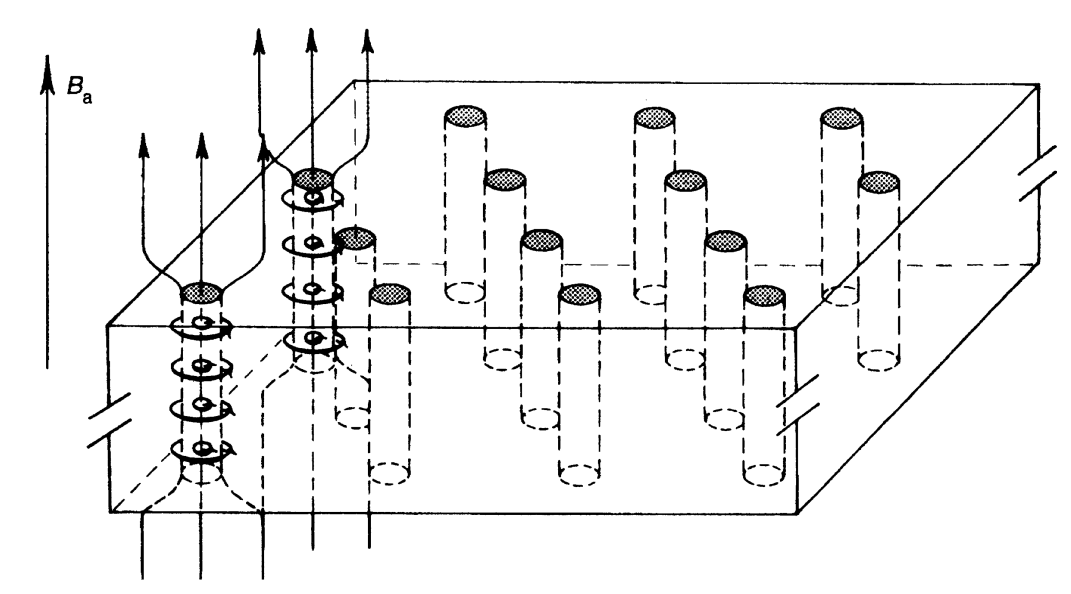
\includegraphics[width=0.7\textwidth]{abbildungen/typ2_supraleiter.png}
% \caption[Versuchsplatz]{\textbf{Flussfadengitter in einem Typ II-Supraleiter [\ref{ref:mappe}].} Magnetfelder treten durch Kanäle in den Supraleiter ein. Die Flüsse sind quantisiert und verlaufen entlang der Magnetfeldrichtung.}
% \label{fig:typII}
% \end{figure}


% \subsection{YBCO}

% Der Supraleiter Yttrium-Barium-Kupferoxid $\mathrm{YBa}_2 \mathrm{Cu}_3 \mathrm{O}_{7-x}$ (\textbf{YBCO}) ist ein Hochtemperatursupraleiter.
% Die kritische Temperatur beträgt 
% \begin{equation}
% T_\mathrm{C} = \SI{93}{K} ~.
% \end{equation}
% Es ist ein harter Supraleiter zweiter Art, der Flussfäden fest einfriert.
% Die Kristallstruktur ist Perowskitartig und abhängig von einer wohlgeordneten Struktur.

\FloatBarrier
\subsection{Funktionsweise eins RF-SQUIDs}
Ein sogenanntes SQUID (\emph{superconducting quantum interference device}) 
ist ein Gerät zur Detektion von kleinsten Änderungen in
magnetischen Feldern. 
Hier werden wir ein  in diesem Versuch verwendetes, sogenanntes RF-SQUID beschreiben, 
das mit einem Wechselstrom betrieben wird.
Es besteht aus einem supraleitenden Ring, der eine dünne, nicht-supraleitende Schwachstelle besitzt. 
Gerät das SQUID nun in ein externes Magnetfeld,
so wird in dem Ring ein Kompensationsstrom induziert,
der den magnetischen Fluss durch den Ring auf ein ganzzahliges 
Vielfaches des Flussquants $\Phi_0$ reduziert oder erhöht.

Bei Änderungen des äußeren Magnetfeldes um mehr als ein Flussquant übersteigt der Kompensationsstrom beim SQUID eine kritische Stromdichte und die Supraleitung bricht zusammen, 
sodass der Strom wieder durch Elektronen getragen wird und es zu 
Energieverlusten kommt.

Ein RF-SQUID ist induktiv an ein Wechselfeld gekoppelt, 
meist mit einer Frequenz von einigen 100\,MHz,
mit welchem durch Wechselfelder in Resonanz ein externer Wechselstrom in dem SQUID induziert wird, welcher den Kompensationsstrom überlagert, sodass es periodisch zwischen dem supraleitenden Zustand und dem normalleitenden Zustand, bei dem Energie verbraucht wird, 
hin und her wechselt. 
Die verbrauchte Energie wird dabei dem Schwingkreis entnommen,
der dadurch gedämpft wird, sodass an ihm die Spannungsamplitude abnimmt. 
Aus dieser Spannungsänderung kann dann die Änderung des Magnetfeldes bestimmt werden.
Da man in der Praxis meist mit Magnetfeldern arbeitet, 
die deutlich größer sind als ein Flussquant, 
muss das SQUID als Nulldetektor betrieben werden,
indem man externe Feldänderungen mit einer Spule ausgleicht,
die mit einem Gegenkopplungs-Gleichstrom betrieben wird. 
Dieser ist propotional zu externen Feldänderungen, welche damit nun in einem großen Bereich bestimmt werden können.


In unserem Versuch wird ein 
SQUID der Firma \emph{Jülicher SQUID GmbH} verwendet,
das auf dem Hochtemperatursupraleiter
Yttrium-Barium-Kupferoxid (\emph{YBCO}) mit einer kritischen
Temperatur $T_\mathrm{C} = \SI{93}{K}$ basiert.


% \begin{figure}[tb!]
% \centering
% 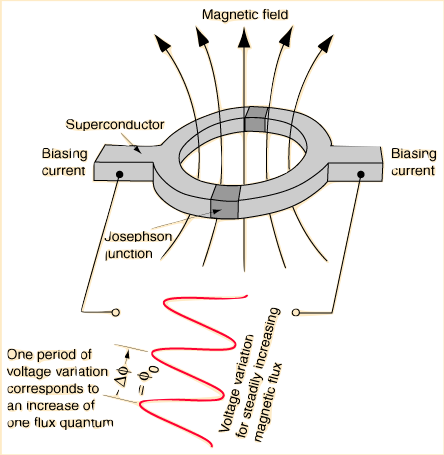
\includegraphics[width=0.5\textwidth]{abbildungen/squide.png}
% \caption[Versuchsplatz]{\textbf{Aufbau eines dc-SQUIDs [\ref{ref:wuppertal}].} An einem supraleitendem Ring mit zwei Josephson-Kontakten wird ein Wechselstrom angelegt. 
% Dieser induziert ein Magnetfeld durch den Ring. 
% Ist das Magnetfeld zu stark, bricht die Supraleitfähigkeit zusammen.
% Diese Änderung im Widerstand kann mit einem Resonanzkreis genau gemessen werden.}
% \label{fig:squid_wuppertal}
% \end{figure}


% \begin{figure}[tb!]
% \centering
% 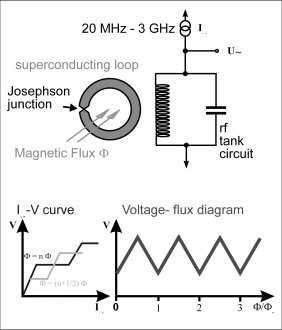
\includegraphics[width=0.4\textwidth]{abbildungen/squid_rf.png}
% \caption[Versuchsplatz]{\textbf{Schema des rf-SQUIDs mit Kennlinien [\ref{ref:jsq}].} Das rf-SQUID wird mit einem Tank-Schwingkreis gekoppelt. Links unten ist die Abhängigkeit der gemessenen Spannung an dem Tankschwingkreis über den Pumpstrom aufgetragen. Rechts unten ist die Fluss zu Spannungs-Transferfunktion abgebildet.}
% \label{fig:jsq}
% \end{figure}


% Angelegt wird eine hochfrequente Spannung von einigen \SI{100}{MHz}. 
% Ein Tank-Schwingkreis ist induktiv mit der SQUID-Schleife gekoppelt und regt diese zur Schwingung an.
% Es gilt für den magnetischen Fluss 

% \begin{equation}
% \Phi_{\mathrm{rf}} = M_\mathrm{G} \cdot Q \cdot I_{\mathrm{rf}} \cdot \sin(\omega_\mathrm{0} t) ~.
% \end{equation}

% $Q$ bezeichnet die Güte des Systems
% \begin{equation}
% Q = \frac{R_\mathrm{T}}{\omega_\mathrm{0} \cdot L_\mathrm{T}} ~.
% \end{equation}
% Die Gegeninduktivität ist mit den Induktivitäten $L_{\mathrm{SQ}}$ und $L_{\mathrm{T}}$ für SQUID-, bzw. Tankschwingkreis,
% \begin{equation}
% M_\mathrm{G} = k \cdot \sqrt{L_{\mathrm{SQ}} \cdot L_\mathrm{T}} ~.
% \end{equation}
% $k$ ist eine Koppelkonstante, $\omega_\mathrm{0}$ die Resonanzfrequenz und $R_\mathrm{T}$ der Widerstand des Tankkreises.

% Gemessen wird die Amplitude der Erregerspannung $\Updelta U_{\mathrm{mess}}$.
% Diese steigt mit $I_{\mathrm{rf}}$ linear an, solange der kritische Strom $I_\mathrm{C}$ von dem Suprastrom durch den SQUID $I_mathrm{S}$ nicht überschritten wird.
% Wird der krtische Strom erreicht nd damit der kritische Fluss $\Phi_\mathrm{C}$, besitzt die Spannung einen kritischen Wert 
% \begin{equation}
% U_{\mathrm{C}} = \frac{\omega_\mathrm{0} \cdot L_\mathrm{T}}{M} ~.
% \end{equation}

% Der Supraleiter wird lokal normalleitend und der Schwingkreis verliert Energie an die Umgebung. 
% Der Verlust beträgt etwa
% \begin{equation}
% \Delta E = I_\mathrm{C} \cdot \Phi_\mathrm{0} ~.
% \end{equation}
% Die Amplitude sinkt drastisch ab und der Vorgang beginnt erneut.


% \section{Versuchsdurchführung}

% Der PC und die benötigte Software (DuoSensor.exe) wird gestartet.
% Mit diesem Programm werden die Werte aufgenommen.
% Die Arbeitspunktjustage wird, falls nicht schon vorhanden, durchgeführt.

% Die Amplitude und Frequenz des Oszillators wird angepasst, sodass die Schwingkreise gekoppelt sind.

\section{Quellen}
\begin{enumerate}
\item Vorbereitungsmappe.\label{ref:mappe}
\item \url{http://hydrogen.physik.uni-wuppertal.de/hyperphysics/hyperphysics/hbase/solids/squid.html} (18.1.2015).\label{ref:wuppertal}
\item \url{http://jsq.apps-1and1.net/category/information/what-is-a-squid/} (18.1.2015).
\label{ref:jsq}
\end{enumerate}



\end{document}
